\chapter{Software}
En este capítulo realizaremos un repaso por las distintas tecnologías de software, y sus características, usadas para la confección de este proyecto. Entre estas tecnologías  se encuentran  varios lenguajes de programación, servidores web, servidores de bases de datos y distintos frameworks.


Para poner un poco de orden, desde el punto de vista del software, podemos distinguir tres bloques claramente diferenciados: la programación de los nodos, el programa servidor y la aplicación de control. Cada uno de ellos usa una combinación distinta de tecnologías para llevar a cabo su función.  Empezaremos desde el nivel más bajo, es decir, la programación de los nodos; para continuar hasta la aplicación de control, el nivel mas alto, la parte que interactúa con el usuario.
 
\section{Programación de los nodos}
Como ya se vio en el anterior capítulo, nuestra elección para los nodos es un Arduino UNO. 

Arduino dispone de un sencillo entorno de desarrollo que permite escribir programas, compilarlos y transferirlos al hardware. Al igual que el resto del entorno  Arduino, se  puede acceder al código fuente, el cual esta escrito en C, C{}\verb!++! y Java.

El IDE se compone del propio editor de texto, un conjunto de librerías y las herramientas de compilación y programación necesarias. Esta disponible en los tres sistemas operativos mayoritarios, Windows, Mac Os X y Linux.

El lenguaje de programación de Arduino esta basado en Processing/Wiring, el cual a su vez se basa en C.

\subsection{El lenguaje de Arduino}
En Arduino  el código fuente se escribe en un lenguaje basado en Processing. Este lenguaje es simplemente un conjunto de funciones en C y C++ a las que se puede llamar desde el código.  Todas las construcciones estándar de C y C{}\verb!++! deben trabajar en Arduino.

El entorno de Arduino lleva a cabo algunas transformaciones para asegurarse que el código es formalmente correcto para C o C++. Después pasa al compilador avr-gcc, que trasforma el código a ficheros objeto. Entonces este código se combina  las librerías estándar de Arduino que implementan las funciones básicas como digitalWrite() o Serial.print().

El resultado es un único archivo hexadecimal Intel, que contiene los bytes necesarios para ser guardados en la memoria de programas del chip de la placa Arduino. Este archivo entonces se graba en la placa: transmitiéndolo vía USB o puerto serie, a través del bootloader que lleva incorporado el chip o con hardware de programación externo.

En definitiva, Arduino se programa en C++ con todas las características de este lenguaje: construcciones y estructuras propias del lenguaje, sintaxis, tipos de datos, declaraciones de variables y funciones, incluso punteros. Ademas de las librerías de funciones  propias de Arduino,  para leer  y escribir en los pines, etc... Con la única restricción de seguir una estructura de programa  predefinida.



\subsubsection{Estructura del programa}
En este lenguaje las operaciones de inicialización y ejecución de tareas tienen sus propias estructuras \emph{setup()} y \emph{loop()}. Así la plantilla básica de un programa Arduino seria:

\begin{verbatim}
void setup(){
    ...
}

void loop(){
    ...
}
\end{verbatim}


La primera función, \emph{setup()}, se ejecutará unicamente cuando Arduino arranca. En ella se pueden realizar las tareas de inicialización de dispositivos, pines y datos.

La segunda función, \emph{loop()}, se ejecuta continuamente una vez que ha finalizado la función anterior. En la mayoría de las aplicaciones esta función sera la que contenga la mayor parte del código

\subsubsection{Funciones básicas de Arduino}
En Arduino hay varias funciones predefinidas, tareas comunes que ofrece para que el programador las pueda utilizar. Algunas de las mas comunes son:
\begin{itemize}
    \item Entrada/salida
        \begin{itemize}
            \item Analógicas
                \begin{description}
                    \item[analogRead()] devuelve el valor leído con el convertidor analógico-digital del microcontrolador.
                    \item[analogWrite()] escribe el valor indicado, de tamaño 1 byte, de forma analógica, empleando un modulador PWM.
                    \item[analogReference()] configura el convertidor analógico-digital para usar las referencias por defecto (alimentación), referencias internas o externas (pin AREF).
                \end{description}
            \item Digital
                \begin{description}
                    \item[pinMode()] indica si un determinado pin es de entrada o salida.
                    \item[digitalRead()] devuelve un valor HIGH o LOW correspondiente al nivel del pin indicado.
                    \item[digitalWrite()] saca un nivel de tensión HIGH o LOW por un pin del controlador.
                \end{description}
        \end{itemize}
    \item Tiempo
        \begin{description}
            \item[delay()] realiza un retardo del numero indicado de milisegundos.
            \item[delayMicroseconds()] realiza un retardo del numero indicado de microsegundos.
            \item[millis()] devuelve los milisegundos que han pasado desde que el programa arrancó. Como los tipos de datos tienen un tamaño finito, este valor se desborda, aproximadamente a los 50 días de funcionamiento continuo.
            \item[micros()] devuelve los microsegundos que han pasado desde que el programa arrancó. Se producirá un desbordamiento cada 70 minutos aproximadamente.
        \end{description}
    \item Manipulación de bits y bytes
        \begin{description}
            \item[lowByte()] devuelve el byte de menor peso de una variable de 2 o mas bytes.
            \item[highByte] devuelve el byte de mas peso de una variable de 2 o mas bytes.
        \end{description}
    \item Interrupciones
        \begin{description}
            \item[interrupts()] habilita las interrupciones para realizar tareas en respuesta a determinados eventos.
            \item[noInterrupts()] deshabilita las interrupciones.
            \item[attachInterrupt()] programa una interrupción externa.
        \end{description}
    \item Serial
        \begin{description}
            \item[begin()] inicializa el puerto serie indicando su velocidad.
            \item[print(), println()] envían datos alfanuméricos por el puerto serie.
            \item[available] devuelve el numero de bytes a la espera de leerse en el buffer.
            \item[read()] devuelve un byte leído por el puerto serie, el byte leído se elimina del buffer.
            \item[write()] escribe datos en binario por el puerto serie.
            \item[peek()] lee un byte pero no lo elimina del buffer.
            \item[flush()] limpia los buffers.
            \item[end()] desactiva el puerto serie.
        \end{description}
\end{itemize}

Esto es solo un extracto de las funciones mas comunes incluidas en las librerias de Arduino. Gracias a la comunidad de Arduino y a la filosofía de código abierto, se puede encontrar una gran cantidad de librerias. Lo que permite no tener que reinventar la rueda cada vez que se quiera utilizar un dispositivo nuevo y aprovechar el trabajo de la comunidad.

Algunas librerias destacadas son:
\begin{description}
    \item[Serial] manejo del puerto serie.
    \item[Software Serial] puerto serie por software.
    \item[Wire] manejo del bus I2C.
    \item[SPI] manejo del bus SPI.
    \item[EEPROM] acceso a nivel de bytes de la memoria EEPROM del microcontrolador
    \item[SD] manejo de memorias SD card para leer y escribir.
    \item[LiquidCrystal] controlar pantallas LCD.
    \item[TFT] controlar pantallas TFT con texto e imágenes.
    \item[Servo] control de motores servo.
    \item[Stepper] control de motores paso a paso.
    \item[GSM] comunicacion en redes GSM o SPRS usando el shield GSM.
    \item[Ethernet] conexiones a Internet a través del shield Ethernet.
    \item[WiFi] conexiones a Internet a través del shield WiFi.
\end{description}


\section{Servidor}
Este programa es la piedra angular del proyecto. Básicamente su función consiste en conectar la red de sensores con la aplicación de usuario. Se encarga de recibir las peticiones de la aplicación de control, pasar estas a la red y recabar y almacenar la información de los sensores. 

Debido a las características y funciones tan especificas del programa, este se desarrollará desde cero. Para ello necesitamos un lenguaje de programación con, al menos, las siguientes características:
\begin{description}
    \item[Soporte multihilo] Para poder atender varias peticiones simultaneas de forma eficiente.
    \item[Soporte para comunicaciones por puerto serie] La comunicación con la red de sensores se realiza mediante este método.
    \item[Soporte para Raspberry Pi] Puesto que es el dispositivo donde se ejecutará, seria deseable que las características únicas de esta placa estén soportadas.
 \end{description}
 
 Por todo lo anterior y su valor educativo, el lenguaje elegido es Python. 
 
 
 \subsection{Python}
 
  Python es un lenguaje de programación creado por Guido van Rossum a principios de los años 90 cuyo nombre está inspirado en el grupo de  cómicos ingleses “Monty Python”. Con una sintaxis muy limpia y que favorece un código legible.
  
  Se trata de un lenguaje interpretado o de script, con tipado dinámico, fuertemente tipado, multiplataforma y orientado a objetos. Su sintaxis simple, clara y sencilla; el tipado dinámico, el gestor de memoria, la gran cantidad de librerías disponibles y la potencia del lenguaje, entre otros, hacen que desarrollar una aplicación en Python sea sencillo y rápido.
  
  La sintaxis es tan sencilla y cercana al lenguaje natural que los programas elaborados en Python parecen pseudocódigo. Por este motivo se trata además de uno de los lenguajes con la curva de aprendizaje mas suaves.
  
  
  Algunos casos de éxito en el uso de Python son Google, Yahoo, la NASA,  y todas las distribuciones Linux, en las que Python cada vez representa un tanto por ciento mayor de los programas disponibles.  
 
 Entre las numerosas características del lenguaje podemos destacar:
 
 \begin{description}
     \item[Lenguaje interpretado o de script] Un lenguaje interpretado o de script es aquel que se ejecuta utilizando un programa intermedio llamado intérprete, en lugar de compilar el código a lenguaje máquina que pueda comprender y ejecutar directamente una computadora (lenguajes compilados).
     
     La ventaja de los lenguajes compilados es que su ejecución es más rápida. Sin embargo los lenguajes interpretados son más flexibles y más portables.
     
     Python tiene, no obstante, muchas de las características de los lenguajes compilados, por lo que se podría decir que es semi interpretado. En Python, como en Java y muchos otros lenguajes, el código fuente se traduce a un pseudo código máquina intermedio llamado bytecode la primera vez que se ejecuta, generando archivos .pyc o .pyo (bytecode optimizado), que son los que se ejecutarán en sucesivas ocasiones.
     
     \item[Tipado dinámico] La característica de tipado dinámico se refiere a que no es necesario declarar el tipo de dato que va a contener una determinada variable, sino que su tipo se determinará en tiempo de ejecución según el tipo del valor al que se asigne, y el tipo de esta variable puede cambiar si se le asigna un valor de otro tipo.
     
     \item[ Fuertemente tipado] No se permite tratar a una variable como si fuera de un tipo distinto al que tiene, es necesario convertir de forma explícita dicha variable al nuevo tipo previamente. Por ejemplo, si tenemos una variable que contiene un texto (variable de tipo cadena o string) no podremos tratarla como un número. En otros lenguajes el tipo de la variable cambiaría para adaptarse al comportamiento esperado.
     
     \item[Sintaxis] Python fue diseñado para ser leído con facilidad. Una de sus características es el uso de palabras donde otros lenguajes utilizarían símbolos. Por ejemplo, los operadores lógicos !, || y \&\& en Python se escriben not, or y and, respectivamente.
     
     El contenido de los bloques de código (bucles, funciones, clases, etc...) es delimitado mediante espacios o tabuladores, conocidos como indentación, antes de cada línea de órdenes pertenecientes al bloque. Python se diferencia así de otros lenguajes de programación que mantienen como costumbre declarar los bloques mediante un conjunto de caracteres, normalmente entre llaves {}.
     
     \item[Multiplataforma] El intérprete de Python está disponible en multitud de plataformas (UNIX, Solaris, Linux, DOS, Windows, OS/2, Mac OS, etc...) por lo que si no utilizamos librerías específicas de cada plataforma nuestro programa podrá correr en todos estos sistemas sin grandes cambios.
     
     \item[Orientado a objetos] La orientación a objetos es un paradigma de programación en el que los conceptos del mundo real relevantes para nuestro problema se trasladan a clases y objetos en nuestro programa. La ejecución del programa consiste en una serie de interacciones entre los objetos.
     
     Python también permite la programación imperativa, programación funcional y programación orientada a aspectos.
     
     \item[Biblioteca estándar] Python tiene una gran biblioteca estándar, usada para una diversidad de tareas. Esto viene de la filosofía <<pilas incluidas>> (<<batteries included>>) en referencia a los módulos de Python. Los módulos de la biblioteca estándar pueden mejorarse por módulos personalizados escritos tanto en C como en Python. Debido a la gran variedad de herramientas incluidas en la biblioteca estándar, combinada con la habilidad de usar lenguajes de bajo nivel como C y C++, los cuales son capaces de interactuar con otras bibliotecas, Python es un lenguaje que combina su clara sintaxis con el inmenso poder de lenguajes menos elegantes.
    \end{description}
    
\section{Aplicación de control}
Esta aplicación es el punto de entrada de usuario al sistema. Para su desarrollo hemos optado por el modelo de aplicación web, ya que necesitamos que esta aplicación se pueda acceder desde cualquier punto de la vivienda, independientemente del dispositivo o sistema operativo usado. Este modelo es el que mejor se adapta a nuestras necesidades.

Más detalladamente sus ventajas son:
\begin{description}
    \item[Instalación] No hace falta instalar nada en los dispositivos cliente, ni la aplicación, ni archivos adicionales. Basta con tener un navegador.
    \item[Compatibilidad] Es completamente compatible con cualquier dispositivo o sistema operativo gracias a los estándares.
    \item[Multiplataforma] Al solo necesitar un navegador, la aplicación es independiente de plataforma y dispositivo.
    \item[Portable] Al ejecutarse sobre un servidor web, cambiar la máquina servidora es tan sencillo como instalar un servidor web en la máquina destino.
    \item[Acceso Inmediato] Pueden ser accedidas desde cualquier dispositivo conectado a la red desde donde se accede a la aplicación. 
    \item[Menos requerimientos de hardware] Este tipo de aplicación no consume (o consume muy poco) espacio en disco del cliente y también es mínimo el consumo de memoria RAM en comparación con las instaladas localmente.
\end{description}


En este modelo de desarrollo es necesario contar con una serie de elementos. Estos son:
\begin{itemize}
    \item Servidor web.
    \item Servidor de bases de datos.
    \item Lenguaje del lado servidor.
     \item Lenguajes del lado cliente.
   \end{itemize}
La combinación específica de los tres primeros se conoce como <<stack>>. 

Para el proyecto hemos elegido el stack LAMP (Linux, Apache, MySQL y PHP), este es uno de los mas populares, probados y robustos que se pueden encontrar. Incluye: Apache como servidor web, MySQL para el manejo de las bases de datos, y PHP como lenguaje del lado del servidor.

Para los lenguajes del lado del cliente de la aplicación usaremos la combinación básica de aplicaciones web, HTML, CSS y Javascript; en sus últimas revisiones. 

\subsection{Servidor web, Apache}
Apache es un servidor de web. Un servidor web es un software que responde a las solicitudes de los navegadores web. En estos momentos, Apache es uno de los servidores web más populares del mundo. Ello se debe, entre otras cosas, a que Apache es un software de alta calidad y de código abierto (open source), lo que significa que puede descargarse de forma gratuita desde Internet.

\begin{figure}[h]
    \centering
    
\includegraphics{imagenes/apache_logo.jpg}
    \caption{Logo del servidor Apache}
    \label{fig:logoapache}
\end{figure}

Apache es uno de los mayores éxitos del software libre y su aceptación entre los servidores web es tan grande que ha llegado hasta el punto de llegar a ser un serio competidor del servidor de web de Microsoft (IIS, Internet information server). Desde 1996, Apache es el servidor web más popular de Internet, hasta llegar a la actual cota de un 68\% de los servidores web frente un 31\% sobre IIS (Fuente: http://news.netcraft.com).

 Su desarrollo es continuo y su portabilidad le ha llevado a plataformas como Windows NT/2000/XP y Windows 95/98/Me,
a los sistemas Unix y a plataformas como MacOS. 

Una de las principales características que presenta Apache es que no solo funciona en la mayoría de las versiones de Unix, sino que, ademas funciona en Windows y en muchos otros sistemas operativos tanto de escritorio como de tipo servidor.

Apache presenta muchas otras características, entre ellas un elaborado indice de directorios; un directorio de alias; negociacion de contenidos; informe de errores HTTP configurable; ejecución SetUID de programas CGI; gestion de recursos para procesos hijos; integracion de imagenes del lado servidor; reescritrura y comprobación ortográfica de URL.

El resto de características importantes de Apache son:

\begin{description}
    \item[Configuración basada en un archivo] El servidor Apache no posee una interfaz de usuario gráfica para su administración. Se trata de un sencillo archivo de configuración llamado <<httpd.conf>>. Únicamente se necesita un editor de texto para configurar el servidor. Sin embargo, es lo suficientemente flexible para permitirle repartir la configuración del host virtual en múltiples archivos para no sobrecargar un único archivo con toda la gestión de las múltiples configuraciones de servidores virtuales.
    
    \item[Soporte para CGI] Apache soporta CGI utilizando los módulos mod\_cgi y \\mod\_cgid. Aporta características extendidas como personalización de las variables de entorno y soporte de reparación de errores o debugging.
    
    \item[Soporte de host virtuales] Apache es ademas uno de los primeros servidores web en soportar tanto host basados en IP como host virtuales.
    
    \item[Soporte de autenticación HTTP] Apache soporta autenticacion basica basada en la web. Esta tambien preparado para autentificación basada en la digestión de mensajes.
    
   \item[Soporte de scripts PHP] Apache ofrece un amplio soporte de PHP mediante el modulo mod\_php.
   
   \item[Soporte de Secured Socket Layer(SSL)] Se puede crear fácilmente un sitio web con SSL utilizando OpenSSL y el modulo mod\_ssl.
\end{description}




\subsection{Servidor de bases de datos, MySQL}
MySQL es un sistema de gestión de bases de datos (SGBD) SQL que en algunos aspectos es aproximadamente tan potente como Oracle. Cabe mencionar que a mediados del año 2009, Oracle, adquirió MySQL.



Sus principales objetivos han sido la velocidad y la robustez. Es un SGBD sencillo y rápido que se adapta perfectamente a entornos en los que el volumen de datos sea del orden de megabytes (en la documentación se habla de su uso con bases de datos de 50 millones de registros). En la versión 5 de MySQL ha incluido el control de transacciones, procedimientos almacenados y triggers, por lo que ha rellenado el gran hueco que lo diferenciaba de grandes SGBD.




Existen en su versión actual distintos motores de almacenamiento de datos, entre los que destacan MyISAM (permite índices por cadenas completas) y InnoDB (que permite el uso de transacciones) o la incorporación de buffers en memoria que permiten agilizar la respuesta de sus resultados. 

Son muchas las razones para escoger MySQL como solución de misión crítica
para la administración de datos:

\begin{description}
    \item[Coste] El coste de MySQL es gratuito para la mayor parte de los usos.
    \item[Asistencia] Gracias a que es software libre, existe una nutrida y activa comunidad de usuarios de MySQL.
    \item[Velocidad]  MySQL es mucho mas rápido que la mayor parte de sus rivales.
    \item[Funcionalidad] MySQL dispone de muchas de las funciones que exigen los desarrolladores, como compatibilidad completa con ACID,  compatibilidad para la mayor parte de SQL ANSI, volcados online, duplication, funciones SSL e integración con la mayor parte de 10s entornos de programación. Así mismo, se desarrolla y actualiza de forma mucho mas rápida que muchos de sus rivales.
    \item[Portabilidad] MySQL se ejecuta en la inmensa mayoría de sistemas operativos y, la mayor parte de los casos, los datos se pueden transferir de un sistema a otro sin dificultad.
    \item[Facilidad de uso] MySQL resulta fácil de utilizar y de administrar. Gran parte de las viejas bases de datos presentan problemas por utilizar sistemas obsoletos, lo que complica innecesariamente las tareas de administración. Las herramientas de MySQL son potentes y flexibles, sin sacrificar su capacidad de uso.
\end{description}

\begin{figure}[ht]
    \centering
    
\includegraphics[width=0.8\textwidth]{imagenes/logo-mysql.jpg}
    \caption{Logo de MySQL}
    \label{fig:logomysql}
\end{figure}

\subsection{PHP}
PHP corresponde a las iniciales de personal home page tools (herramientas para páginas iniciales personales). Es un lenguaje de programación tipo script para entornos web con unas funciones muy semejantes a las de ASP y JSP, utilizado, sobre todo, en servidores Linux para personalizar la información enviada a los usuarios que acceden a un sitio web. 

\begin{figure}[ht]
    \centering
    
\includegraphics{imagenes/php-big.jpg}
    \caption{Logo de PHP}
    \label{fig:logophpl}
\end{figure}

Desde un punto de vista técnico, es un lenguaje interpretado de alto nivel, similar en construcciones léxicas y sintácticas a C, C++, Java y Perl, por lo que a quienes ya conozcan estos lenguajes les resultará muy fácil comenzar a escribir código PHP.

PHP es un lenguaje incrustado (embedded) en páginas HTML, es decir, es un lenguaje de programación que se introduce dentro de las páginas HTML. El código PHP se interpreta en el lado del servidor de web, desde donde se genera la página HTML solicitada antes de llevar a cabo su transmisión al navegador.

De esta forma, podemos programar aplicaciones asociadas al servidor de web, aumentando, así, la funcionalidad de dicho servidor y convirtiéndolo en un sistema de desarrollo de aplicaciones cliente/servidor mucho más completo.

Su principal objetivo es hacer que desarrolladores de aplicaciones basadas en la web puedan escribir páginas que se generan dinámicamente de una forma sencilla y rápida.

En cuanto a la tecnología del intérprete de PHP, la versión 3 ya era tan rápida como los intérpretes existentes de ASP. Con la versión 4 de PHP, su rendimiento y prestaciones mejoraron todavía más: el intérprete (Zend) era hasta
12 veces más rápido que el de la versión 3; se modularizó todo el diseño interno; se perfeccionó su integración con otros servidores HTTP como el IIS de Microsoft, y se encaró hacia la programación orientada a objetos (Programación OO). 

Con la versión 5, se ha rediseñado completamente el motor Zend, para crear un lenguaje completamente OO, agilizando más aún su funcionamiento, y extrayendo la compatibilidad con MySQL en un módulo externo.

PHP proporciona, por tanto, una gran facilidad para acceder a diferentes tipos de bases de datos como Oracle, Sybase, MySQL, PostgreSQL, Adabas, etc. De hecho, es bastante sencillo portar una aplicación escrita con PHP para MySQL
a cualquier otro servidor de base de datos, ya que las funciones de acceso que ofrece PHP son, en muchos casos, de sintaxis compartida.

\subsubsection{El motor Zend}
El nombre Zend se refiere al motor del lenguaje, es decir, el núcleo de PHP.

El término PHP se refiere al sistema completo tal y como aparece desde fuera. Zend ocupa la parte de intérprete (analiza el código de entrada de un script, lo traduce y lo ejecuta), y también un poco de la parte de funcionalidad (implementa la funcionalidad del sistema). 

PHP ocupa la parte de funcionalidad y la de interfaz (habla con el servidor web, etc.). Juntos forman el paquete completo PHP. Zend forma realmente el núcleo del lenguaje, mientras que PHP contiene todos los módulos externos (los cuales se pueden cargar en tiempo de ejecución) e incorporados (los que se compilan directamente con PHP) que crean las posibilidades destacadas del lenguaje.

\begin{figure}[htp]
    \centering
    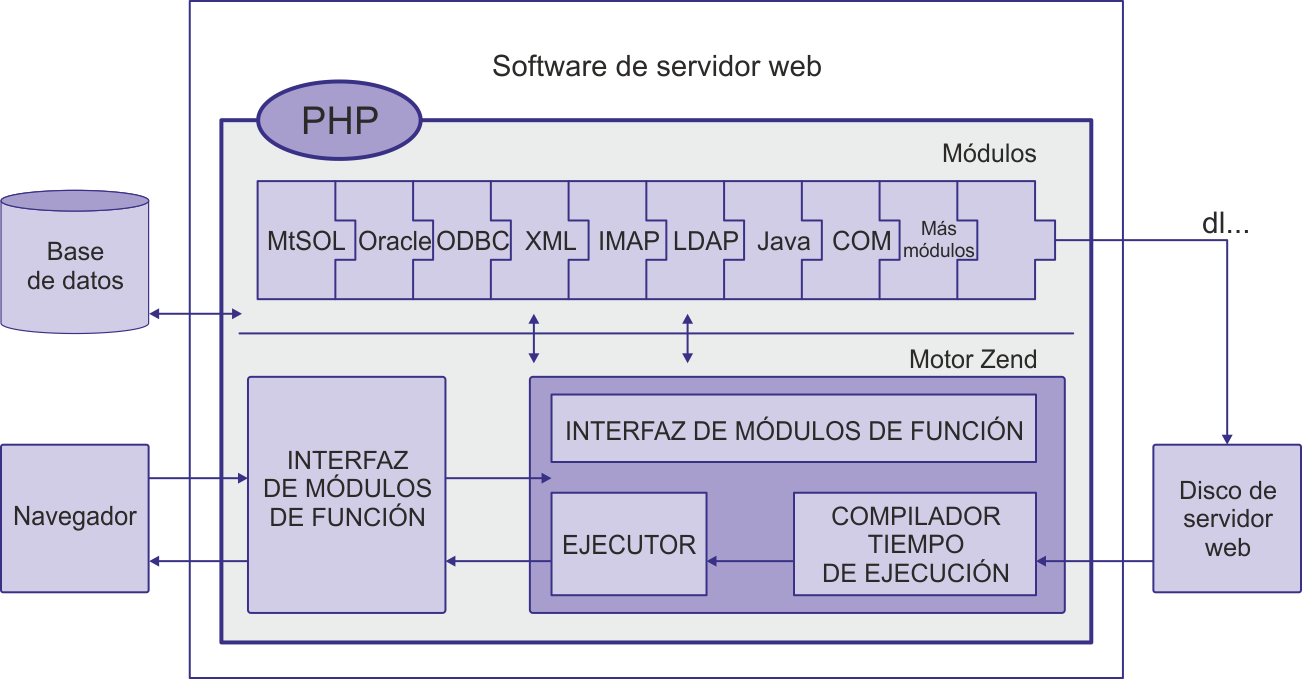
\includegraphics[width=0.8\textwidth]{imagenes/estructura_php.png}
    \label{fig:estructuraphp}
    \caption{Estructura interna de PHP}
\end{figure}



\subsection{HTML 5}[b]
HTML (Hyper Text Markup Language) es el lenguaje usado para escribir las páginas web, describe la estructura y el contenido usando solo texto y lo complementa con objetos tales como imágenes, flash y otros. Los archivos así creados son guardados con la extensión de archivo HTM o HTML.




Su estructura se compone de etiquetas o tags entre las cuales van insertados los diferentes elementos que componen la pagina como son los bloques de texto, scripts y la ruta a la ubicación de archivos externos como imágenes y otros archivos multimedia. El navegador al cargar dichos archivos representa todos los elementos en ella de forma adecuada.

Existen varias versiones o especificaciones de HTML, son las siguientes:
\begin{itemize}
    \item HTML la primera especificación de 1991.
    \item HTML 3.0 propuesta por el recién formado W3C en 1995.
    \item HTML 4 1999.
    \item XHTML 2002.
    \item HTML5 usándose actualmente pero aun en desarrollo.
\end{itemize}

\begin{figure}[hb]
    \centering
    
\includegraphics[width=0.3\textwidth]{imagenes/HTML5-Logo.png}
    \caption{Logo de HTML5}
    \label{fig:logoHTML}
\end{figure}

HTML5 surge como una evolución lógica de las especificaciones anteriores y por la necesidad de lograr los siguientes objetivos:
\begin{itemize}
    \item Lograr que la información, y la forma de presentarla estén lo más separadas posible.
    \item Resumir, simplificar y hacer más sencillo el código utilizado.
    \item Un lenguaje que haga las páginas compatibles con todos los navegadores web, incluyendo los de los teléfonos móviles y otros dispositivos modernos usados en la actualidad para navegar en Internet.
    \item Eliminar restricciones que hagan el código más popular y asequible.
\end{itemize}

\subsubsection{Principales estándares en el lenguaje HTML}

HTML4
Posiblemente el lenguaje mas usado en las paginas de Internet es el HTML4, a pesar de estar ya casi obsoleto debido a sus limitaciones.
Muchos CMS, están diseñados para crear las paginas usando dicha especificación, por lo que se siguen sumando muchas de ellas a los millones acumuladas en los servidores de Internet.
Una página escrita en HTML4 puede ser que se muestre de forma diferente en distintos navegadores, o que no se muestre en lo absoluto.
Es imposible representar en dicho lenguaje multitud de caracteres especiales como los Unicode, que son tan comunes en las páginas.

XHTML
Después del HTML4 surge el XHTML en dos versiones, Transitional y Strict, lenguaje desde sus inicio considerado de transición y de uso temporal, no obstante representa un adelanto enorme respecto a las posibilidades que introduce, limitado siempre al tratar de mantener la compatibilidad con la especificación anterior. 
Es más ligero y compatible con cualquier navegador, su desventaja es que posee muchas restricciones, por lo que muchos no se habituaron fácilmente al salto que representó su introducción y aun siguen atrapados en el lenguaje anterior.

HTML5
Finalmente llega HTML5, recoge todas las ventajas que introdujo el XHTML y elimina bastante restricciones y limitaciones.
Es más ligero al ser más sencillo y simple el código, lo que permite que las paginas escritas en este lenguaje carguen mas rápido en el navegador.
Si aun no fuera suficiente, introduce infinidad de opciones que hasta ahora estaban vedadas a las páginas web, como insertar directamente vídeo, música, y casi cualquier elemento.

\subsubsection{Novedades de HTML 5}

En términos de Markup, el HTML5 introduce algunos elementos que hacen que se adecue a los tiempos que corren. Así, muchas de las novedades están relacionadas con la forma de construir websites que se tiene en la actualidad. Una de las más importantes novedades está relacionada con la inserción de multimedia en los sitios web, que ahora contarán con etiquetas HTML especiales para poder ser incluidos. Por otro lado, algunos aspectos de diseño también son incluidos en el lenguaje, así como también algunos detalles de navegación.

Con el uso de HTML5, se puede reducir la dependencia de los plug-ins que tenemos que tener instalados para poder ver una determinada web. Caso emblemático, el de Adobe Flash, que se ve claramente perjudicado por la instauración de este estándar. Por otro lado, fue un avance importante para dispositivos que de forma nativa no soportaban Flash, y que no soportaban tampoco plug-ins necesarios para hacerlo. Pero además, con HTML5 se amplía el horizonte del desarrollo de aplicaciones que pueden ser usadas en una multiplicidad de dispositivos.

Gracias a HTML5, los usuarios pueden acceder a sitios web de manera offline, sin estar conectados a internet. Se suma también la funcionalidad de drag and drop, y también la edición online de documentos ampliamente popularizada por Google Docs. La geolocalización es uno de sus puntos fuertes, pero por otro lado, las etiquetas diseñadas especialmente para el audio y el vídeo ahorran la necesidad de tener que tener un plug-in.

\subsubsection{Las nuevas etiquetas}
El lenguaje HTML funciona a través de marcas de sentido llamadas etiquetas. Las etiquetas son la herramienta fundamental para que los navegadores puedan interpretar el código y permitirnos ver imágenes, texto, párrafo, y estructuras. Los navegadores vendrían a ser como “traductores” de las etiquetas, y con HTML5, se agregan nuevas etiquetas para utilizar que nos ahorran el uso de otros productos que se usaban para complementar y hacer cosas que con el simple HTML no se podían hacer. 

HTML5 fue creado para hacer que el proceso de escribir el código sea más simple y más lógico, por decirlo de una forma. La sintaxis de HTML5 se destaca, como dijimos, en el ámbito multimedia, pero son bastantes las etiquetas introducidas para generar una mejoría.

La idea detrás de HTML5 es que podamos visualizar el contenido multimedia variado que podemos encontrar en Internet aún cuando nos encontramos en dispositivos de gama baja que no podrían soportarlo. No solamente contamos con etiquetas especiales como audio, vídeo y canvas, sino también integración con contenidos de gráficos en vectores (que anteriormente se conocía como la etiqueta object). Con estas etiquetas, los usuarios pueden consumir vídeos y canciones, por ejemplo, sin necesidad de instalar nada de forma adicional.

Las más importantes de las nuevas etiquetas creadas son:

\begin{description}
    \item[article] esta etiqueta sirve para definir un artículo, un comentario de usuario o una publicación independiente dentro del sitio.
    \item[nav] la negación puede ser insertada directamente en el markup, entre estas etiquetas, que nos permitirán hacer que nuestras listas oficien de navegación.
    \item[section] con esta etiqueta, una de las más importantes de las novedades, se puede definir todo tipo de secciones dentro de un documento. Por ponerlo de forma sencilla, funciona de una forma similar a la etiqueta div que nos separa también diferentes secciones.
    \item[embed] con esta etiqueta se puede marcar la presencia de un contenido interactivo o aplicación externa.
    \item[header, footer] estas etiquetas individuales ahorran tener que insertar IDs para cada uno, como se solía hacer anteriormente. Además, se pueden insertar headers y footers para cada sección, en lugar de tener que hacerlo únicamente en general.
    \item[audio y video] estas son las dos más importantes etiquetas de HTML5, dado que nos permiten acceder de forma más simple a contenido multimedia que puede ser reproducido por casi todo tipo de dispositivos; marcan el tipo de contenido que estará en su interior.
    \item[canvas] finalmente, esta etiqueta nos permite introducir un “lienzo” dentro de un documento, para poder dibujar gráficos por vectores; será necesario el uso de JavaScript.
\end{description}

Hay otras etiquetas inauguradas por HTML5 pero destacamos estas por la innovación que introducen en nuestro código. 

Las etiquetas a las que estábamos acostumbrados, por otro lado, introducen un nuevo funcionamiento. El caso ejemplo es el de las etiquetas header y footer, que, como dijimos, ahora permiten separar las secciones, y no solamente el comienzo y el fin de una página.

El funcionamiento del DOCTYPE también se renueva, siendo mucho más simple de usar y menos engorroso. 

\subsection{CSS 3}

El CSS es un lenguaje de estilos empleado para definir la presentación, el formato y la apariencia de un documento de marcaje, sea html, xml, o cualquier otro. Comúnmente se emplea para dar formato visual a documentos html o xhtml que funcionan como espacios web. También puede ser empleado en formatos xml, u otros tipos de documentos de marcaje para la posterior generación de documentos.

\begin{figure}[htb]
    \centering
    
\includegraphics[width=0.3\textwidth]{imagenes/css3logo.png}
    \caption{Logo de CSS 3}
    \label{fig:logocss}
\end{figure}

Las hojas de estilos nacen de la necesidad de diseñar la información de tal manera que podemos separar el contenido de la presentación y, así, por una misma fuente de información, generalmente definida mediante un lenguaje de marcaje, ofrecer diferentes presentaciones en función de dispositivos, servicios, contextos o aplicativos. Por lo que un mismo documento html, mediante diferentes hojas de estilo, puede ser presentado por pantalla, por impresora, por lectores de voz o por tabletas braille. Separamos el contenido de la forma, composición, colores y fuentes.

La especificación de CSS está mantenida por el World Wide Web Consortium (W3Cg).


Las diferentes revisiones de las hojas de estilo tienen el origen en la primera especificación publicada por el W3C en diciembre de 1996 y que pretendía unificar la sintaxis y el modo de definir una hoja de estilos por los diferentes lenguajes derivados del SGML. Así, las principales características que se pueden definir mediante esta primera especificación son:
\begin{itemize}
    \item Propiedades del tipo de letra, así como el estilo de este.
    \item Colores de los textos y de los fondos.
    \item Atributos del texto tales como espacio entre caracteres, palabras y líneas.
    \item Alineación de tablas, bloques de texto, imágenes, párrafos.
    \item Márgenes externos e internos, filetes y posición de la mayoría de los elementos.
    \item Definición única de elementos mediante ids y agrupamiento de atributos
    mediante classes.
\end{itemize}

A partir de esta primera especificación, en mayo de 1998, y como una extensión a la primera revisión, aparece la segunda, popularmente conocida como la especificación CSS2, y adoptada por la mayoría de los navegadores. 

Como características fundamentales que añade la revisión, se encuentra la posibilidad de definir posiciones de forma absoluta, relativa y fija, así como la profundidad de los elementos (z-index) cuando existen superposiciones, también el soporte para formatos de voz y textos bidireccionales. De esta, aparece una revisión, la 2.1, que incorpora muchas de las mejoras hechas por los fabricantes de navegadores y que actualmente es empleada y estandarizada.

La tercera revisión de la especificación del CSS por el W3C empieza en el 2005 y todavía está en proceso de definición. Pero esta vez, las diferentes implementaciones de los motores de renderizado de los navegadores no están esperando a tener una especificación, sino que implementan ciertas cosas a su manera y, por lo tanto, muchas son utilizables en entornos de producción web. 

Es necesario, sin embargo, partir siempre de la consideración de que las diferentes implementaciones de los navegadores no es exacta, y de que, por lo tanto, cuando diseñamos una hoja de estilos, el principio que tiene que regir es que funcione en todas partes, y no que funcione igual.

A diferencia de las otras especificaciones, esta vez se ha dividido en temas. De este modo disponemos de diferentes temas que pueden crecer y evolucionar en paralelo, y no como uno grande y monolítico, con muchísimas revisiones (cada vez hay más gente interesada y evoluciona más deprisa).

Así, en la nueva revisión encontramos grupos como el de selectores, unidades de medida, modelo de caja, colores y gamas, modelo de línea, texto, fuentes, lenguajes verticales, page-media... entre otros. Y de este modo, diferentes módulos tienen un estatus diferente y son adoptados por los fabricantes de software a diferente velocidad.

A grandes rasgos podemos destacar dos beneficios del uso de CSS3
\begin{description}
    \item[Reducción del tiempo de desarrollo y mantenimiento] Utilizar propiedades y métodos de CSS3 puede ser un beneficio directo a la hora
    de desarrollar, puesto que nos ahorramos bastante trabajo, como por ejemplo
    a la hora de hacer fondo con esquinas redondeadas. Antes había que hacerlo
    con imágenes. También ahorramos mucho trabajo a la hora de hacer
    sombras, ya que nos ahorramos de nuevo la imagen que teníamos que usar
    antes (normalmente un gráfico en formato png).
    También podemos mejorar el rendimiento al tener menos código, divs dentro
    de divs, etc.
    \item[Incremento del rendimiento de las páginas] Menos etiquetas html indican\\ menos código a la hora de descargarse del servidor  y menos código a la hora de interpretar y dibujar el navegador. Dos ahorros, uno de ancho de banda y el otro de rendimiento del ordenador. Además, muchas de las técnicas de CSS3 nos ahorran imágenes, que a la vez cumplen la doble premisa de rendimiento.
\end{description}



Las novedades de CSS3 con respecto a las versiones anteriores incluyen:
\begin{description}
    \item[Nuevos selectores] Los selectores CSS son la herramienta más potente del lenguaje de estilos, puesto que nos permiten seleccionar diferentes elementos del contenido html en función de la etiqueta o de sus atributos sin tener que hacer uso de su clase, su ID o Javascript.
    \begin{itemize}
        \item Selectores de atributos.
        \item Pseudo-clases.
        \item Pseudo-elementos.
        \item ...
    \end{itemize}
    
    \item[Colores RGBA] La posibilidad de especificar colores en modo RGB ya existía desde la especificación 2, pero en la versión 3 se ve ampliada con un nuevo modelo de color, el basado en saturación (HSL), y la posibilidad de especificar canal alpha sobre
    los colores.
    
    \item[Colores HSL] El modelo de color HSL (hue, saturation, light), tono, saturación y luz; define el color a partir de estos tres parámetros. Así, para una tonalidad de color dada, podemos alterar la saturación a partir del segundo parámetro, y la cantidad de  luz en el tercer parámetro.
    
    \item[Opacidad] Como su nombre indica, la opacidad nos permite definir el nivel de transparencia para un selector. A diferencia del modelo RGB, la transparencia se aplica
    al objeto y todos sus hijos y/o contenidos.
    
    \item[Esquinas redondeadas] Seguramente es la propiedad CSS3 más esperada y deseada por los diseñadores html. Permite redondear las esquinas de una caja (div, span... ) dado un radio, sin la necesidad de usar nada más.
    
    \item[Sombras, en cajas y texto] En la versión 2 de la especificación se introdujo la posibilidad de generar sombras directamente desde código CSS, pero se quitó en la 2.1 y se ha vuelto a introducir en la versión 3.
    
    \item[Webfonts] Otra de las posibilidades que resulta muy atractiva a la hora de emplear los CSS3 es la capacidad de adjuntar tipografías a un documento html. A partir de la especificación 3, disponemos de la etiqueta @font-face, que nos permite definir una tipografía.
    
    \item[MediaQueries] Desde la versión 2.1 de los CSS, existe la posibilidad de definir estilos en función del uso de la hoja: una para la pantalla (screen), otra para la impresión (print), otra para los lectores de voz (voice). A partir de la especificación 3 esto va un paso más allá, y nos permite definir estilos específicos para diferentes tamaños de pantalla. La posibilidad de poder trabajar así, realmente, nos ofrece soluciones óptimas, puesto que podemos emplear sólo CSS para crear una versión móvil de un site.
\end{description}


\subsection{Javascript}

Javascript es un lenguaje de programación que surgió con el objetivo inicial de programar ciertos comportamientos sobre las páginas web, respondiendo a la interacción del usuario y la realización de automatismos sencillos. En ese contexto podríamos decir que nació como un <<lenguaje de scripting>> del lado del cliente, sin embargo, hoy Javascript es mucho más. Las necesidades de las aplicaciones web modernas y el HTML5 ha provocado que el uso de Javascript que encontramos hoy haya llegado a unos niveles de complejidad y prestaciones tan grandes como otros lenguajes de primer nivel.

Pero además, en los últimos años Javascript se está convirtiendo también en el lenguaje <<integrador>>. Lo encontramos en muchos ámbitos, ya no solo en Internet y la Web, también es nativo en sistemas operativos para ordenadores y dispositivos, del lado del servidor y del cliente. La visión de Javascript <<como lenguaje para crear pequeños programas dentro del ámbito de una página web>> se ha quedado muy pequeña.

En el contexto de un sitio web, con Javascript se puede hacer todo tipo de acciones e interacción. Antes se utilizaba para validar formularios, mostrar cajas de diálogo y poco más. Hoy es el motor de las aplicaciones más conocidas en el ámbito de Internet: Google, Facebook, Twitter, Outlook...

A Javascript se le denomina <<del lado del cliente>> porque donde se ejecuta es en el navegador (cliente web), en contraposición a lenguajes como PHP que se ejecutan del <<lado del servidor>>. 

En Javascript, es el navegador el que soporta la carga de procesamiento. Gracias a su compatibilidad con todos los navegadores modernos se ha convertido en un estándar como lenguaje de programación del lado del cliente.

Con Javascript podemos crear y definir interacciones con el usuario. El navegador del cliente es el encargado de interpretar las instrucciones Javascript y ejecutarlas para realizar estas interactividades, de modo que el mayor recurso, con que cuenta este lenguaje es el propio navegador y todos los elementos que hay dentro de una página. Pero ahora, gracias a las API Javascript de HTML5, que están disponibles en los navegadores actuales de ordenadores y dispositivos, podemos acceder a todo tipo de recursos adicionales, como la cámara, espacio para almacenamiento de datos, creación de gráficos basados en vectores y mapas de bits, flujos de datos con servidores, etc. Con todo ello se han multiplicado las posibilidades.


JavaScript es un lenguaje de programación interpretado, dialecto del estándar ECMAScript. Se define como orientado a objetos, basado en prototipos, imperativo, débilmente tipado y dinámico.

JavaScript se diseñó con una sintaxis similar al C, aunque adopta nombres y convenciones del lenguaje de programación Java. Sin embargo Java y JavaScript no están relacionados y tienen semánticas y propósitos diferentes.

Las propiedades más importantes de JavaScript son las siguientes:
\begin{itemize}
    \item Se interpreta por el ordenador que recibe el programa, no se compila.
    \item Tiene una programación orientada a objetos. El código de los objetos está predefinido y esexpandible. No usa clases ni herencia.
    \item El código está integrado (incluido) en los documentos HTML.
    \item Trabaja con los elementos del HTML.
    \item No se declaran los tipos de variables.
    \item Ejecución dinámica: los programas y funciones no se chequean hasta que se ejecutan.
    \item Es orientado a eventos, los programas se ejecutan cuando sucede algo, un evento.
\end{itemize}

La sintaxis de JavaScript es muy similar a la de otros lenguajes de programación como Java y C. Las normas básicas que definen la sintaxis de JavaScript son las siguientes:
\begin{description}
    \item[No se tienen en cuenta los espacios en blanco y nuevas líneas] Como sucede con XHTML, el intérprete de JavaScript ignora cualquier espacio en blanco sobrante, por lo que el código se puede ordenar de forma adecuada para entenderlo mejor (tabulando las líneas, añadiendo espacios, creando nuevas líneas, etc...)
    
    \item[Se distinguen las mayúsculas y minúsculas] Al igual que sucede con la sintaxis de las etiquetas y elementos XHTML. Sin embargo, si en una página XHTML se utilizan indistintamente mayúsculas y minúsculas, la página se visualiza correctamente, siendo el único problema la no validación de la página. En cambio, si en JavaScript se intercambian mayúsculas y minúsculas el script no funciona.
    
    \item[No se define el tipo de las variables] Al crear una variable, no es necesario indicar el tipo de dato que almacenará. De esta forma, una misma variable puede almacenar diferentes tipos de datos durante la ejecución del script.
    
    \item[No es necesario terminar cada sentencia con el carácter ;] En la mayoría de lenguajes de programación, es obligatorio terminar cada sentencia con el carácter ;. 
        
    \item[Se pueden incluir comentarios] Los comentarios se utilizan para añadir información en el código fuente del programa. Aunque el contenido de los comentarios no se visualiza por pantalla, si que se envía al navegador del usuario junto con el resto del script, por lo que es necesario extremar las precauciones sobre la información incluida en los comentarios.
\end{description}

\section{Frameworks}

El concepto framework se emplea un muchos ámbitos del desarrollo de sistemas software, no solo en el ámbito de aplicaciones Web. Podemos encontrar frameworks para el desarrollo de aplicaciones médicas, de visión por computador, para el desarrollo de juegos, y para cualquier ámbito que pueda ocurrírsenos.

En general, con el término framework, nos estamos refiriendo a una estructura software compuesta de componentes personalizables e intercambiables para el desarrollo de una aplicación. En otras palabras, un framework se puede considerar como una aplicación genérica incompleta y configurable a la que podemos añadirle las últimas piezas para construir una aplicación concreta. 

Los objetivos principales que persigue un framework son: acelerar el proceso de desarrollo, reutilizar código ya existente y promover buenas prácticas de desarrollo como el uso de patrones.

El objetivo principal de todo framework es facilitar las cosas a la hora de desarrollar una aplicación, haciendo que nos centremos en el verdadero problema y nos olvidemos de implementar funcionalidades que son de uso común.

El uso de un framework a la hora de realizar un proyecto, ofrece importantes ventajas, ventajas ya no sólo al facilitarnos la tarea de la creación de la aplicación, sino otras como en el mantenimiento del código, realizar ampliaciones, etc...

Otras ventajas son:
\begin{description}
    \item[Uso de patrones de diseño] Uno de las principales ventajas que ofrecen los framework es el uso de patrones de diseño para el desarrollo de la aplicación. El patrón más utilizado y que casi todos los framework utilizan es el conocido como Modelo – Vista – Controlador (MVC).
    
    \item[Estructura predefinida de la aplicación] El programador no necesita plantearse la estructura global de la aplicación, ya que esta es proporcionada por el  framework. Tiene la ventaja de que pasado un tiempo, si hay  que tocar algo en la aplicación, sabremos donde encontrar el archivo en cuestión de forma rápida.
    
    \item[Código altamente testeado] Todo el código que forma parte del framework está altamente probado, lo que garantiza el buen    funcionamiento del mismo. Se podría desarrollar esas mismas funcionalidades, pero   nunca podremos garantizar el nivel de testeo que ofrece un framework.
    
    \item[Comunidad de usuarios detrás de cada framework] La gran mayoría de los frameworks tienen detrás a una amplia comunidad de usuarios, de los    cuales muchos ayudan en su desarrollo o creando extensiones con funcionalidades extra que podremos utilizar de forma sencilla sin tener que desarrollarlas por nuestra cuenta.
\end{description}

\subsubsection{Patrón MVC, Modelo Vista Controlador}

Para comprender como trabajan los frameworks Web existentes es imprescindible conocer el patrón MVC.

El patrón Modelo-Vista-Controlador es una guía para el diseño de arquitecturas de aplicaciones que ofrezcan una fuerte interactividad con usuarios. Este patrón organiza la aplicación en tres modelos separados, el primero es un modelo que representa los datos de la aplicación y sus reglas de negocio, el segundo es un conjunto de vistas que representa los formularios de entrada y salida de información, el tercero es un conjunto de controladores que procesa las peticiones de los usuarios y controla el flujo de ejecución del sistema.

El modelo MVC puede ser implementado sin la necesidad de utilizar un framework, pero la diferencia radica en que el framework nos obliga a utilizarlo, creando de esta forma un código mucho más robusto. 

Además el uso de este tipo de utilidades nos ayuda a evitar el conocido como <<código spaghetti>>, que consiste en meter funcionalidades en capas que no corresponde, lo que con el paso de tiempo hará que nuestro código sea un verdadero caos.

La mayoría, por no decir todos, de los framewroks para Web implementan este patrón. 


Algunas caracteristicas presentes en casi todos los frameworks web son:
\begin{description}
    \item[Abstracción de URLs y sesiones] No es necesario manipular directamente las URLs ni las sesiones, el framework ya se encarga de hacerlo. 
    
    \item[Acceso a datos] Incluyen las herramientas e interfaces necesarias para     integrarse con herramientas de acceso a datos, en BBDD,
    XML, etc... 
    
    \item[Controladores] La mayoría de frameworks implementa una serie de     controladores para gestionar eventos, como una     introducción de datos mediante un formulario o el acceso a     una página. Estos controladores suelen ser fácilmente     adaptables a las necesidades de un proyecto concreto. 
    
    \item[Autentificación y control de acceso] Incluyen mecanismos para la identificación de usuarios mediante login y password y permiten restringir el acceso a     determinas páginas a determinados usuarios. 
   
    \item[Internacionalización]
    
    \item[Separación entre diseño y
    contenido]
\end{description}

En la realización de este proyecto se ha incorporado diversos frameworks. Principalmente dos:
\begin{itemize}
    \item Laravel, para PHP.
    \item Bootstrap, para CSS.
\end{itemize}

\subsection{Laravel}
Durante varios años PHP se ha ganado una mala reputación entre los desarrolladores que tuvieron que mantener aplicaciones desarrolladas sin ningún tipo de estructuración.

Pasó el tiempo y apareció el proyecto Symfony, el cual está basado en los principios de crear un desarrollo más sólido flexible y testeable, algo que las aplicaciones PHP no tenían.

Laravel nace confiando en Symfony, pero también depende de otras grandes librerías como SwiftMailer, Carbon o Doctrine, es decir, se ha tomado la mejor de los grandes para hacer un framework muy robusto.

Laravel se apoya en las mejoras introducidas en las últimas versiones de PHP como pueden ser:
\begin{description}
    \item[Espacios de nombres (namespaces)] Se utilizan extensivamente en lenguajes como Java y evitan la colisión de nombres cuando el mismo nombre de función se utiliza en diferentes librerías. Los espacios de nombres se separan mediante “\\”, y éstos se deben replicar en la estructura del directorio. Se declaran en la parte superior del archivo tomando una estructura como . 
    \begin{verbatim}
        <?php 
        namespace Illuminate\Database\Eloquent
        ?>
    \end{verbatim}
    Para indicar los espacios de nombres en los que PHP deberá buscar las clases, utilizamos la palabra “use” seguida del espacio de nombre de la clase, por ejemplo: \verb|use Illuminate\Database\Eloquent\Model|.
    \item[Interfaces (interfaces)]  También se conocen como Contratos y son una forma de definir los métodos que una clase deberá proveer, si implementa esa interfaz. Las Interfaces no contiene ningún detalle de implementación, únicamente son contratos.
    
    \item[Funciones anónimas] Ayudan a crear código más corto y se utilizan para definir rutas, eventos, filtros y en otras partes. Ejemplo de una función anónima en una ruta: \verb|Route::get(‘hi’, function(){ return ‘hi’;});|
    
    \item[Sobrecarga (overloading)] También llamados métodos dinámicos o mágicos, nos permiten llamar a métodos que no estaban previamente definidos en una clase. Ejemplo: \verb|whereUsernameOrEmail ($name, $email)|.  
    
    Estas llamadas se manejan con el método \verb| _call()|, el cual trata de pasear el nombre para ejecutar uno o más de los métodos conocidos. En este caso \verb|->where(‘usuario’, $usuario)->orWhere(‘email’,$email)|.


\end{description}

\begin{figure}[htb]
    \centering
    
\includegraphics[width=0.8\textwidth]{imagenes/laravel-logo.png}
    \caption{Logo de Laravel}
    \label{fig:logolaravel}
\end{figure}

Laravel: Principales características y fuentes de inspiración

\subsubsection{Principales características}

Veamos qué es lo que se puede esperar de un proyecto con Laravel y como éstas características pueden ayudar a incrementar la productividad:

\begin{description}
    \item[Modularidad] Laravel se ha construido utilizando más de 20 librerías diferentes fuertemente integradas con el gestor de dependencias Composer.
    
    \item[Testeabilidad] Construido para facilitar el testeo, Laravel tiene con varios asistentes (helpers) que ayudan a visitar las rutas de testeo, navegando por el HTML resultante para asegurar que los métodos que se llaman desde las diferentes clases sean correctos, e incluso a impersonar a los usuarios.
    
    \item[Enrutamiento (routing)] Laravel proporciona un extrema flexibilidad en la definición de las rutas de la aplicación. Inspirado en la filosofía de los micro-frameworks Sinatra y Silex. Todavía más, es posible adjuntar funciones de filtro que se ejecuten en rutas específicas.
    
    \item[Gestor de configuración] Frecuentemente la aplicación se ejecutará en diferentes entornos, esto quiere decir que tanto la base de datos como credenciales o dominios serán diferentes si se ejecutan el local en el entorno de test o en los servidores de producción. Laravel nos permite definir configuraciones separadas para cada uno de los entornos.
    
    \item[Confeccionador de consultas y ORM] Cuando se instala Laravel viene con un constructor de consultas, este nos permite lanzar consultas a la base de datos con una sintaxis PHP de métodos enlazados, en lugar de tener que escribir la SQL completa. Además proporciona un ORM y una implementación de RegistroActivo (ActiveRecord) llamado Eloquent, que permite definir modelos interconectados. Estos componentes son compatibles con bases de datos tales como PostgreSQL, SQLite, MySql, MS SQL Server.
    
    \item[Confeccionador esquema, migraciones y repoblaciones] Inspirado por la filosofía Rails, estas características permiten definir un esquema de base de datos dentro de PHP y mantener un registro de los cambios para así ayudar en la migración de base de datos. Las repoblaciones (Seeding) permiten poblar las tablas seleccionadas de una base de datos una vez realizada la migración para de esta forma rellenar con datos las tablas.
    
    \item[Motor de plantillas] Laravel viene con Blade, un lenguaje ligero de plantillas con el cual se pueden crear diseños anidados con bloques predefinidos en el que el contenido se inserta dinámicamente. Además Blade guarda en caché los archivos generados.
    
    \item[Autenticación] Laravel viene con las herramientas para crear en toda web un formulario de registro, autenticación e incluso envio de contraseñas a usuarios que no la recuerden.
    
    \item[Redis] Es un sistema de almacenamiento clave-valor en memoria que tiene fama de ser extremadamente rápido.
    \item[Colas] Laravel se integra con diversos servicios de colas, tales como Amazon SQS o IronMQ, para permitir el aplazamiento de tareas que son muy intensivas en recursos, así por ejemplo podemos enviar una gran cantidad de e-mails ejecutando esta tarea en segundo plano en lugar de hacer que el usuario espere delante de la pantalla.
\end{description}

\subsubsection{Simplicidad en la sintaxis}

El corazón de la filosofía de Laravel es la simplicidad y la expresividad. Esto quiere decir que los desarrolladores de Laravel han dado especial atención en el nombrado de las clases para comunicar con efectividad las acciones en un inglés sencillo.

Observemos el siguente trozo de código:

\begin{verbatim}

<? php
Route:: get(' area/{ id}', function( $ id){
    if( 51 = = $ area and !Auth:: check()) {
        return Redirect:: guest(' login');
    } else {
    return “Bienvenido a tu parte ”. $area;
}
})->where (‘id’,’[0-9]+’);

\end{verbatim}

A simple vista nos podemos  hacer una idea de lo que  hace este código. Eso es expresividad, hacer que el código sea más legible, con lo que probablemente también será  un codigo más sencillo y menos propenso a errores.




\subsection{Bootstrap}

Twitter Bootstrap es un framework o conjunto de herramientas de software para diseño de sitios y aplicaciones web. Contiene plantillas de diseño con tipografía, formularios, botones, cuadros, menús de navegación y otros elementos de diseño basado en HTML y CSS, así como, extensiones de JavaScript opcionales adicionales.

Es el proyecto más popular en GitHub y es usado por la NASA y la MSNBC junto a más organizaciones.

Bootstrap fue desarrollado por Mark Otto y Jacbod Thornton de Twitter, como framework para fomentar la consistencia a través de herramientas internas. Antes de Bootstrap, se usaban varias librerías para el desarrollo de interfaces de usuario, las cuales guiaban a inconsistencias y a una carga de trabajo alta en su mantenimiento. 

Según el desarrollador de Twitter Mark Otto, frente a esos desafíos:
\begin{quotation}
    ...un pequeño grupo de desarrolladores y yo nos reunimos a diseñar y construir una nueva herramienta interna y vimos una oportunidad de hacer más. A través de ese proceso, nos vimos construir algo mucho más sustancial que otra herramienta interna más. Meses después, terminamos con una primera versión de Bootstrap como una manera de documentar y compartir bienes y patrones de diseño comunes dentro de la compañía.
\end{quotation}

En agosto del 2011, Twitter liberó a Bootstrap como código abierto.


\subsubsection{Características}
Bootstrap tiene un soporte relativamente incompleto para HTML5 y CSS 3, pero es compatible con la mayoría de los navegadores web. La información básica de compatibilidad de sitios web o aplicaciones esta disponible para todos los dispositivos y navegadores. Existe un concepto de compatibilidad parcial que hace disponible la información básica de un sitio web para todos los dispositivos y navegadores. Por ejemplo, las propiedades introducidas en CSS3 para las esquinas redondeadas, gradientes y sombras son usadas por Bootstrap a pesar de la falta de soporte de navegadores antiguos. Esto extiende la funcionalidad de la herramienta, pero no es requerida para su uso.

Desde la versión 2.0 también soporta diseños responsables. Esto significa que el diseño gráfico de la página se ajusta dinámicamente, tomando en cuenta las características del dispositivo usado (PCs, tabletas, teléfonos móviles).


Bootstrap viene con una disposición de cuadricula estándar de 940 píxeles de ancho para posicionar los elementos de la aplicacion o pagina web. Aparte, también tiene cuatro variaciones para hacer uso de distintas resoluciones y tipos de dispositivos: teléfonos móviles(formato vertical y apaisado), tabletas y computadoras con baja y alta resolución. Esto ajusta el ancho de las columnas automáticamente.

También proporciona un conjunto de definiciones básicas de estilo para todos los componentes de HTML. Esto otorga uniformidad al visualizar la aplicacion en cualquier navegador y sistema.

Como añadido a los elementos principales de HTML, Bootstrap contiene otra interfaz de elementos comúnmente usados. Ésta incluye botones con características avanzadas (e.g grupo de botones o botones con opción de menú desplegable, listas de navegación, etiquetas horizontales y verticales, ruta de navegación, paginación, etc.), etiquetas, capacidades avanzadas de miniaturas tipográficas, formatos para mensajes de alerta y barras de progreso.

Los componentes de JavaScript para Bootstrap están basados en la librería jQuery de JavaScript. Los plug-ins proveen elementos adicionales de interfaz de usuario como diálogos, tooltips y carruseles. También extienden la funcionalidad de algunos elementos de interfaz existentes, incluyendo, por ejemplo, una función de auto-completar para campos de entrada (input). 

\subsubsection{Estructura y Función}
Bootstrap es modular y consiste esencialmente en una serie de hojas de estilo LESS que implementan la variedad de componentes de la herramienta. Una hoja de estilo llamada bootstrap.less incluye los componentes de las hojas de estilo. Los desarrolladores pueden adaptar el mismo archivo de Bootstrap, seleccionando los componentes que deseen usar en su proyecto.

Los ajustes son posibles en una medida limitada a través de una hoja de estilo de configuración central. Los cambios más profundos son posibles mediante las declaraciones LESS.

El uso del lenguaje de hojas de estilo LESS permite el uso de variables, funciones y operadores, selectores anidados, así como clases mixins.

Desde la versión 2.0, la configuración de Bootstrap también tiene una opción especial de <<Personalizar>> en la documentación. Por otra parte, los desarrolladores eligen en un formulario los componentes y ajustes deseados, y de ser necesario, los valores de varias opciones a sus necesidades. El paquete consecuentemente generado ya incluye la hoja de estilo CSS pre-compilada.
















